\myChapter{Results}
\label{chap:results}

% \section{Numerical results}
% \label{sec:numerical-results}


% \section{Visual results}
% \label{sec:numerical-results}

In this section we present the results in terms of inference speed and image quality using plain PyTorch implementations of UNet and SRUNet, and their compiled versions with TensorRT, using fp32, fp16, and int8 precisions for weights/activations.

\begin{table*}[t]
\begin{tabular}{llllll}
\toprule
{} &          lpips &           ssim &            psnr &        ms\_ssim &         brisque \\
\midrule
unet        &  0.559 ± 0.007 &  0.879 ± 0.004 &  21.939 ± 0.027 &  0.735 ± 0.002 &   153.591 ± 0.0 \\
unet\_fp32   &  0.354 ± 0.011 &  0.897 ± 0.003 &   28.64 ± 0.108 &  0.871 ± 0.003 &   26.783 ± 1.83 \\
unet\_fp16   &  0.354 ± 0.011 &  0.897 ± 0.003 &   28.64 ± 0.108 &  0.871 ± 0.003 &   26.788 ± 1.84 \\
unet\_int8   &  0.343 ± 0.011 &  0.895 ± 0.003 &  28.613 ± 0.108 &   0.87 ± 0.003 &  26.448 ± 1.694 \\
srunet      &  0.551 ± 0.008 &  0.869 ± 0.004 &  19.303 ± 0.014 &  0.669 ± 0.002 &   153.591 ± 0.0 \\
srunet\_fp32 &  0.396 ± 0.012 &  0.896 ± 0.003 &  28.837 ± 0.126 &  0.871 ± 0.003 &  34.647 ± 2.336 \\
srunet\_fp16 &  0.396 ± 0.012 &  0.896 ± 0.003 &  28.837 ± 0.126 &  0.871 ± 0.003 &  34.642 ± 2.334 \\
srunet\_int8 &  0.373 ± 0.012 &  0.895 ± 0.003 &  28.806 ± 0.124 &  0.869 ± 0.003 &  34.868 ± 1.989 \\
\bottomrule
\end{tabular}
\caption{Averages (± standard deviations) of IQA metrics for different variations of UNet and SRUNet implementations.}
\label{tab:tab1}
\end{table*}

\Cref{tab:tab1} shows the average value of each IQA metric for each model variation, along with the standard deviation (shown as ±). The values in the table indicate the quality of the images generated by the models, with higher values indicating better quality.
LPIPS and Brisque metrics underline strong differences between plain PyTorch implementations and their relative TRT ones for both UNet and SRUNet, the same can be said of psnr, while ssim and ms\_ssim stay in the same range of values for each model variation.

\begin{table*}[t]
\begin{tabular}{ll}
\toprule
{} &      times [s] \\
\midrule
unet        &    0.035 ± 0.0 \\
unet\_int8   &    0.015 ± 0.0 \\
unet\_fp16   &  0.028 ± 0.001 \\
unet\_fp32   &  0.028 ± 0.001 \\
srunet      &    0.012 ± 0.0 \\
srunet\_int8 &    0.006 ± 0.0 \\
srunet\_fp16 &    0.009 ± 0.0 \\
srunet\_fp32 &  0.009 ± 0.001 \\
\bottomrule
\end{tabular}
\caption{Averages (± standard deviations) of evaluation times in seconds for different variations of UNet and SRUNet implementations.}
\label{tab:tab2}
\end{table*}

\Cref{tab:tab2} shows the execution times (in seconds) of different variations of UNet and SRUNet implementations. Each table entry represents the average execution time over more than 300 executions "±" its standard deviation. SRUNet generally has faster execution times than UNet across all numerical precisions. Among the different numerical precisions, the fastest execution times are generally achieved, as expected by using int8, followed by fp16 and fp32.

TODO: make figure captions shorter and describe such images.

\begin{figure*}[h]
  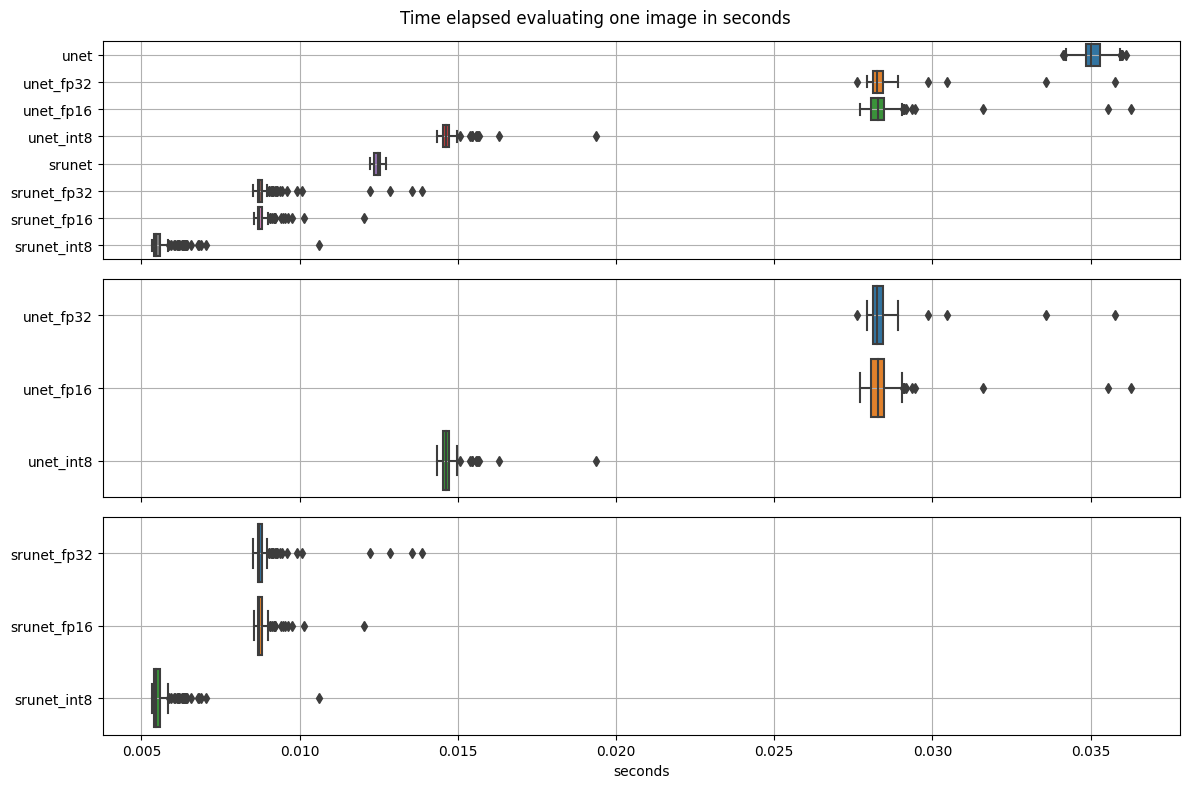
\includegraphics[width=1.0\textwidth]{static/2023_03_02_boxplots_timings_all.png}
  \caption{Average times elapsed in seconds for generating one image using different versions of UNet and SRUNet implementations. The top graph shows all the versions, the middle one zooms in comparing only the TRT versions of UNet, as well as the bottom graph for SRUNet.}
\end{figure*}

\begin{figure*}[h]
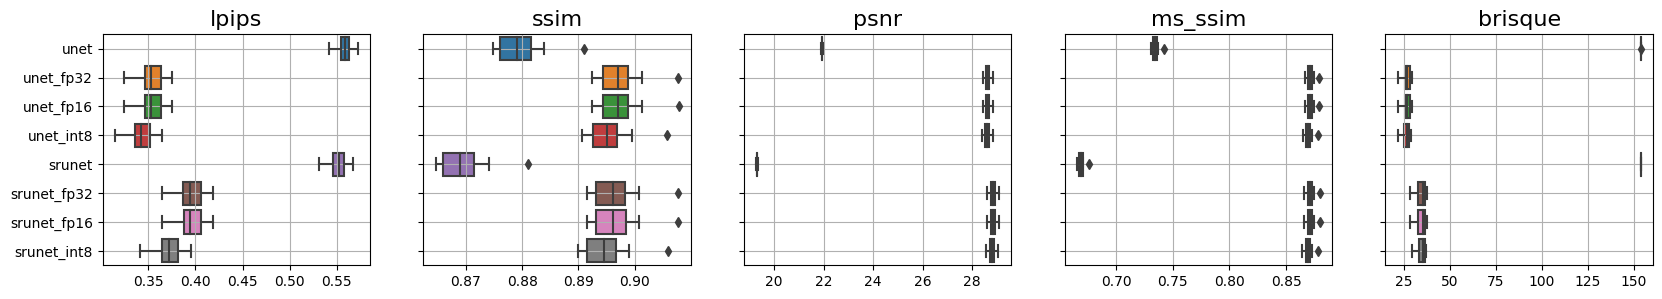
\includegraphics[width=1.0\textwidth]{static/2023_03_02_boxplots_metrics_all.png}
\caption{Average results for some IQA metrics on validation images with different versions of UNet and SRUNet implementations.}
\end{figure*}

\begin{figure*}[h]
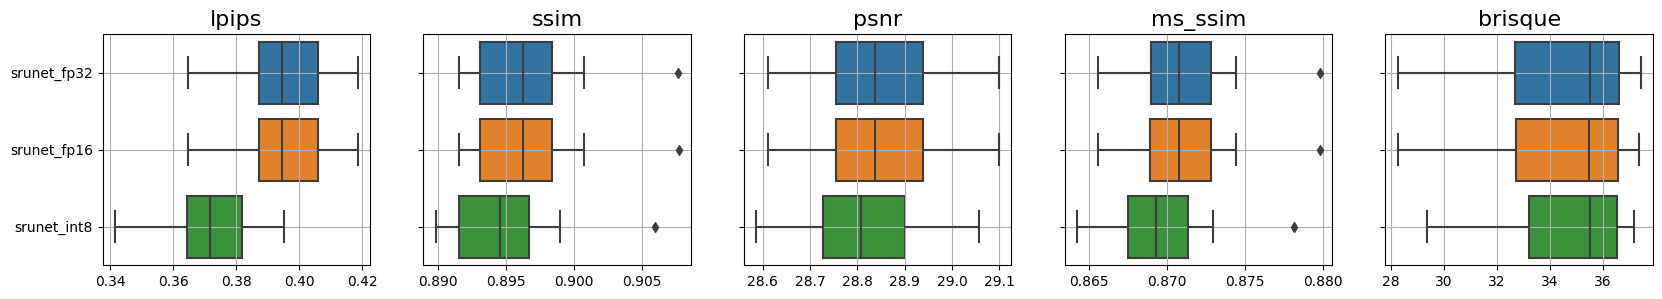
\includegraphics[width=1.0\textwidth]{static/2023_03_02_boxplots_metrics_quant_srunet.png}
\caption{Average results for some IQA metrics on validation images with different versions of UNet implementations.}
\end{figure*}

\begin{figure*}[h]
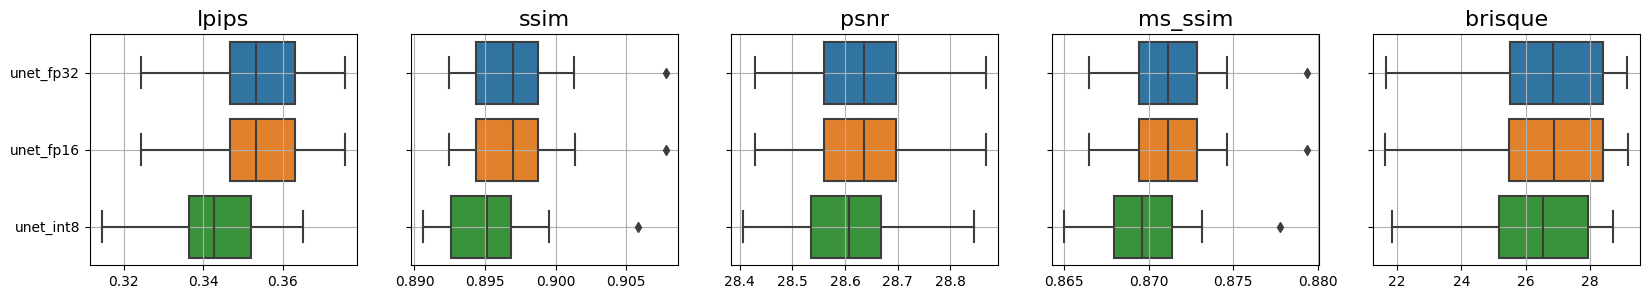
\includegraphics[width=1.0\textwidth]{static/2023_03_02_boxplots_metrics_quant_unet.png}
\caption{Average results for some IQA metrics on validation images with different versions of SRUNet implementations.}
\end{figure*}

